\subsection{Accuracy Evaluation}
\label{subsec:accuracy}

To validate the accuracy of \vmps, we have implemented a dedicated
version of our
framework\footnote{\url{https://github.com/BeyondTheClouds/G5K-VMPlaceS}}
on top of the Grid'5000 testbed and compared the execution of the
Entropy strategy invoked every 60 seconds over a 3600 seconds period
in both the simulated and the real world.  Regarding the
\textit{in-vivo} conditions, experiments have been performed on top of
the Graphene cluster (Intel Xeon X3440-4 CPU cores, 16 GB memory, a
GbE NIC, Linux 3.2, Qemu 1.5 and SFQ network policy enabled) with 6
VMs per node.  Each VM has been created using one of 8 VM predefined
classes. The template was 1:1GB:1Gbps:1Gbps:X, where the memory update
speed X was a value between 0 and 80\% of the migration bandwidth
(1Gbps) in steps of 10. Starting from 0\%, the load of each VM varied
according to the exponential and the Gaussian distributions. The
parameters were $\lambda$ = \#VMs/300 and $\mu$= 60, $\sigma$ = 20.
Concretely, the load of each VM varied on average every 5 min in steps
of 10 (with a significant part between 40\% and 80\%). A dedicated
\texttt{memtouch} program~\cite{Hirofuchi:2013:ALM:2568486.2568524}
has been used to stress both the CPU and the memory
accordingly. Regarding the simulated executions, \vmps has been
configured to reflect the \textit{in-vivo} conditions. In particular,
we configured the network model of SimGrid in order to cope with the
network performance of the Graphene servers that were allocated to our
experiment (6 MBytes for the TCP gamma parameter and 0.88 for the
bandwidth corrective simulation factor).

Fig.~\ref{fig:usecase-vivosimu} shows the cost of the two phases of
the Entropy algorithm for each invocation when considering 32~PMs and
192~VMs through simulations (top) and in reality (bottom). Overall, we can see that simulation results successfully
followed the in-vivo ones. During the first hundreds seconds, the cluster did not
experience VM requirement violations because the loads of VM were
still small (\ie Entropy simply validated that the current placement
satisfied all VM requirements). At 540 seconds, Entropy started to
detect non viable configurations and performed reconfigurations.
Diving into details, the difference between the \textit{simulated} and
\textit{in-vivo} reconfiguration time fluctuated between 6\% and 18\%
(median was around 12\%). %during the experiment.
The worst case, \ie 18\%, was reached when
multiple migrations were performed simultaneously on the same
destination node.
%\begin{figure}[hbt]
\begin{wrapfigure}{r}{.48\linewidth}
\centering
\vspace*{-.7cm}
%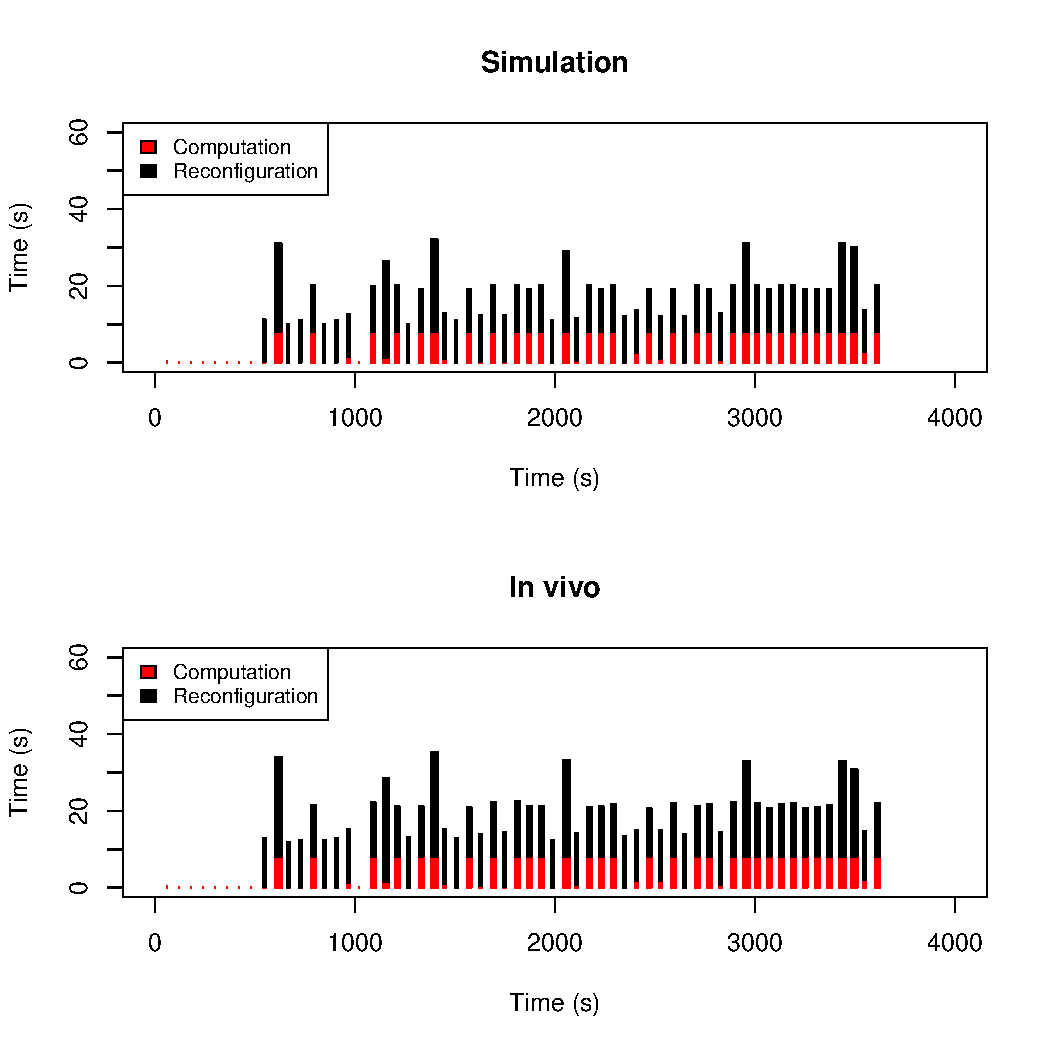
\includegraphics[width=0.99\linewidth]{./figures/simu-vivo-32PM-192VM-6020-original.pdf}
 \subcapcentertrue
\subfigure{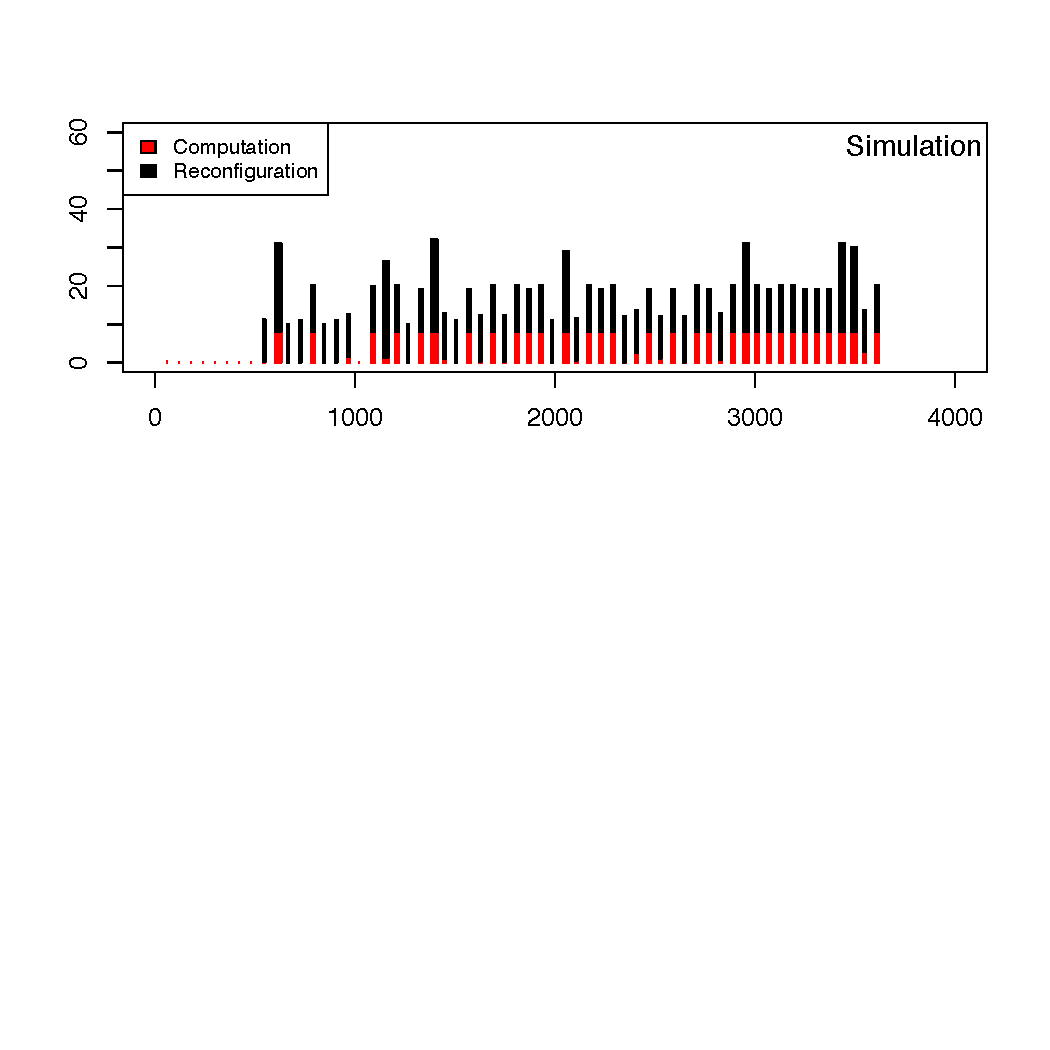
\includegraphics[width=0.99\linewidth]{./figures/accuraci-simu.pdf}
\label{fig:accu-simu}}
\subfigure{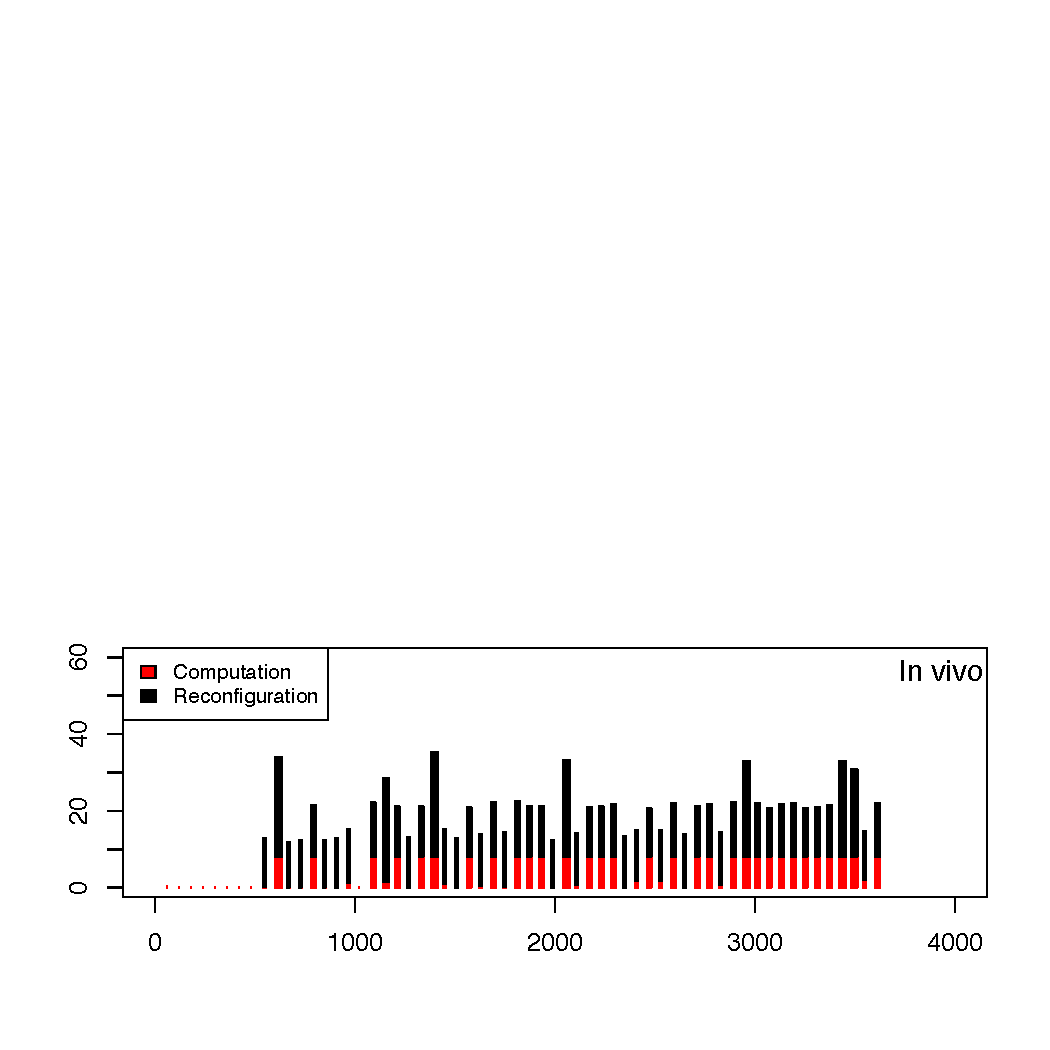
\includegraphics[width=0.99\linewidth]{./figures/accuraci-invivo.pdf}
\label{fig:accu-vivo}}
\vspace*{-.8cm}
\caption{Comparison between simulated (top) and \textit{in-vivo}
  (bottom) Executions}
\flushleft\scriptsize{The red parts correspond the computation phase (\ie
  the time where Entropy looks for a new configuration). The black parts correspond to the reconfiguration phase (\ie when
VM are relocated throughout the cluster.}
\label{fig:usecase-vivosimu}
\vspace*{-.7cm}
\end{wrapfigure}
%\end{figure}
 In this case and even if the SFQ network policy was
enabled, we discovered that in the reality the throughput of migration
traffic fluctuated when multiple migration sessions simultaneously
shared the same destination node. We confirmed this point by analyzing
TCP bandwidth sharing through \texttt{iperf} executions. We are
currently investigating with the \sg core-developers how we can
integrate this phenomenon into the live-migration model. However, as a
migration lasts less than 15 seconds in average, we believe that that
the current simulation results are sufficiently accurate to capture
performance trends of placement strategies.


% As an example, we noticed that applying the
% reconfiguration plan was much more time-consuming than computing it. This result that has been correctly reported by the simuations means that VMPP also needs
% to address the way of shorten reconfiguration phases, not only that of
% computing ones.
% % This is rather important as most relocation
% % algorithms try to reduce the computation phase instead of focusing on the
% % reconfiguration one.
% Leveraging \vmps will enable researchers to observe such key points
% without facing with the burden of conducting large scale
% \textit{in-vivo} experiments. We illustrate such an advantage in the
% following section.




%%% Local Variables:
%%% mode: latex
%%% TeX-master: "main"
%%% End:
